% ICDE 2027 Research Track manuscript; evidence and build records accompany the source.
\documentclass[conference]{IEEEtran}
\usepackage{amsmath,amssymb,graphicx,booktabs,array,url}
\usepackage[table]{xcolor}
\definecolor{QInk}{HTML}{203449}
\definecolor{QHead}{HTML}{EFF3F7}
\definecolor{QFocus}{HTML}{EDF7F5}
\newcommand{\qth}[1]{\textcolor{QInk}{\textbf{#1}}}
\usepackage[hidelinks]{hyperref}
\newtheorem{theorem}{Theorem}
\newtheorem{proposition}{Proposition}
\newcommand{\E}{\mathbb{E}}
\newcommand{\C}{\mathcal{C}}
\newcommand{\R}{\mathbb{R}}
\newcommand{\qbridge}{Q-BRIDGE}
\title{Q-BRIDGE: Verifiable Policy Queries over Joint Confidence Views}
\hypersetup{pdftitle={Q-BRIDGE: Verifiable Policy Queries over Joint Confidence Views},
pdfauthor={Zida Yang, Weiqing Zeng, Guquan You, Cong Wang, Jiexin Zheng}}
% Latest user-confirmed order and roles: only Cong Wang and Jiexin Zheng correspond.
\author{
\IEEEauthorblockN{\href{https://orcid.org/0009-0000-2386-2533}{Zida Yang}$^{1,\dagger}$,
\href{https://orcid.org/0009-0003-0186-6199}{Weiqing Zeng}$^{2,\dagger}$,
\href{https://orcid.org/0009-0005-5915-7058}{Guquan You}$^{3,\dagger}$,
\href{https://orcid.org/0000-0002-5300-0122}{Cong Wang}$^{1,*}$,
\href{https://orcid.org/0009-0005-5838-0135}{Jiexin Zheng}$^{1,*}$}
\IEEEauthorblockA{$^{1}$Guanghua School of Management, Peking University}
\IEEEauthorblockA{$^{2}$Southwest Jiaotong University}
\IEEEauthorblockA{$^{3}$Institute of Emergency Safety Innovations, Guangzhou University}
\IEEEauthorblockA{2401111090@stu.pku.edu.cn, zengweiqing@my.swjtu.edu.cn, youguquan@gzhu.edu.cn}
\IEEEauthorblockA{\{wangcong,jiexinzheng\}@gsm.pku.edu.cn}
\IEEEauthorblockA{$\dagger$ Equal contribution. \quad $*$ Corresponding authors.}
}

\begin{document}
\maketitle
\begin{abstract}


Recommendation systems often use historical logs and randomized experiments to select policies, rules for assigning items to users, that improve outcomes over a reference. However, observational bias, sampling uncertainty, and limited transfer across populations make policy gains difficult to establish. Evaluating a limited set of candidate policies leaves a decision gap. When none guarantees the desired improvement, it remains unclear whether another policy could meet the target or whether the available evidence rules out such a guarantee for all policies. We treat these decisions as repeated queries over a reusable view of uncertain action outcomes, separating evidence construction from policy choice and query execution. Q-BRIDGE materializes observational intervals and randomized group constraints into a joint confidence view. It supports evaluating individual policies, finding the largest worst-case gain achievable by any policy, and certifying when no policy meets a requested threshold. For disjoint action groups, we develop a three-step algorithm that finds an optimal policy with independently verifiable bounds; exact linear programming handles more general constraints. Our algorithm matches the optimal guarantees computed by exact linear programming across 2,160 synthetic policy optimization problems. In 107 cases where evaluating the original candidate policies leaves the existence of a qualifying policy unresolved, searching the full policy family finds qualifying policies in 86 cases and rules out such guarantees in the remaining 21. Retaining exact certificate terms reduces repeated-query cost. Experiments on the Coat recommendation dataset illustrate how the available evidence can support policy redesign or justify stopping the search.

\end{abstract}
\begin{IEEEkeywords}
query processing, uncertain data, materialized views, causal inference, verifiable computation
\end{IEEEkeywords}

\section{Introduction}
A recommendation analyst often reuses logs and randomized experiments to compare policies~\cite{schnabel2016coat}. Policies assign actions to user groups; gain is expected improvement over a reference. The data stay fixed while the analyst changes the policy or required gain.

Production assignments may reflect unobserved preferences~\cite{Kallus2018ConfoundingRobust}, and experimental results may transfer only at group level~\cite{lanners2025fusion}. Sampling adds uncertainty. These sources permit several possible action-success probabilities. We seek a gain guaranteed across all possibilities consistent with the evidence and source assumptions.

Checking a candidate list leaves a decision gap. If no candidate meets the target, could another policy succeed, or does the available evidence rule out that guarantee for every policy? The answers call for policy redesign or stopping search on the unchanged view.

We develop Q-BRIDGE\footnote{Code and saved certificate examples: \url{https://github.com/yzd2002/Q-BRIDGE-ICDE2027}.}, a query framework that separates evidence construction from policy choice and execution. It materializes observational intervals and randomized group constraints into one \emph{confidence view}. A policy is a linear query; its worst-case gain is the guaranteed answer. Q-BRIDGE also finds the largest guarantee over all policies and certifies when none meets a threshold. Each answer carries evidence checked independently against the stored view.

\textbf{The data engineering problem.} Repeated decisions raise two query-processing questions: which evidence remains valid when objectives change, and which work can be shared? Causal query systems address biased aggregates~\cite{salimi2018hypdb}; uncertainty-annotated databases preserve bounds across queries~\cite{Feng2019UADB}. We connect these concerns through one jointly covered view, a whole-family query operator and exact certificate reuse. Adaptive queries reuse these bounds without rescanning events.

\textbf{Running example.} Figure~\ref{fig:example} compares four jackets A--D for one population. Success means a high rating; $m_A,\ldots,m_D$ are the unknown rates. The reference selects each with probability $1/4$. Logs bound individual rates; transferred experimental group averages give $(m_A+m_C)/2=.65$ and $(m_B+m_D)/2=.70$. The reference's success probability is $(.65+.70)/2=.675$. Since $m_A\le.6$, the first group forces $m_C\ge.7$. Always choosing C guarantees $.7-.675=.025=2.5$\,percentage points (pp). The allowed vector $(.6,.7,.7,.7)$ limits every action to $.7$, ruling out a larger guarantee. Matching bounds proves optimality.

\begin{figure*}[t]
\centering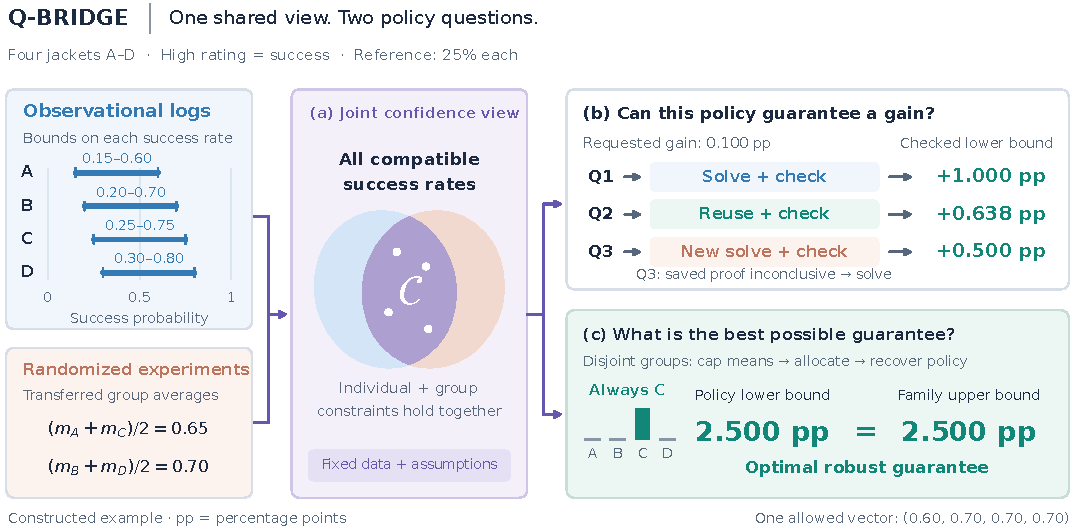
\includegraphics[width=\textwidth]{figures/qbridge_overview.pdf}
\caption{One view, two query paths. Both sources constrain the same success rates; two allowed scenarios illustrate the view. The upper path checks three policies: Q2 reuses Q1's certificate; Q3 needs a new solve. The lower path establishes the best guarantee, 2.5\,pp. This constructed example uses rounded inputs.}
\label{fig:example}
\end{figure*}

Figure~\ref{fig:example} tests a margin $\delta=.001=0.1$\,pp. Section~\ref{sec:reuse} works through these three policies to explain when saved evidence suffices and when a new solve is needed.

\textbf{Materialize evidence once (II--III).} Source summaries and declared assumptions define a shared view. Its joint coverage supports policies chosen after earlier query answers.

\textbf{Answer beyond a candidate list (IV).} For disjoint nonnegative groups, the smallest feasible cap yields an optimal policy and an original-view certificate. Exact LP handles overlaps.

\textbf{Reuse checked work (IV--VI).} Saved certificate terms answer changing objectives in linear arithmetic work. Controlled comparisons separate policy choice, source information and execution cost.

Table~\ref{tab:query-contract} summarizes the interface.
\begin{table*}[t]
\centering
\caption{Three questions over one fixed view. Guarantees concern every allowed mean vector; their failure does not establish a nonpositive actual effect.}
\label{tab:query-contract}
\begin{tabular}{@{}p{.29\textwidth}p{.67\textwidth}@{}}
\toprule
Question & Answer and independently checked evidence \\
\midrule
Does this policy guarantee gain $>\delta$? & True: a lower bound above $\delta$. False: an allowed counterexample. Unknown: neither established. Reuse or solve for this policy; overlapping groups allowed. \\
What is the largest worst-case gain? & Capacity $\mathcal R$ and an attaining policy: its lower bound matches an upper bound for all policies. Our direct construction handles disjoint nonnegative groups; a general exact LP also handles overlaps. \\
Can every such guarantee be ruled out? & Yes, if one allowed mean vector limits even the best policy's gain to $\delta$. No full optimization is needed when this witness suffices. \\
\bottomrule
\end{tabular}
\end{table*}


\section{Policy Queries and Their Guarantees}\label{sec:contract}
We define guaranteed improvement, then the assumptions that turn each source into constraints.
\subsection{The query and the stored object}
Let $X\in\{1,\ldots,K\}$ identify a user group, $A\in\{1,\ldots,L\}$ an action such as recommending a jacket, and $Y\in\{0,1\}$ success. There are $d=KL$ group--action pairs. The potential outcome $Y(a)$ asks whether this user would succeed if given action $a$, even when that action was not observed. Observational source $O$ defines the target population; randomized source $R$ may describe another population. Their means are $m^O_{xa}=\E_O[Y(a)\mid X=x]$ and $m^R_{xa}=\E_R[Y(a)\mid X=x]$.

Policy $\pi_{xa}$ is the probability of taking action $a$ in context $x$; $\pi_0$ is the reference and $w_x$ the target context proportion. The expected gain is
\begin{equation}
 \Delta(c)=\sum_{x,a}w_x(\pi_{xa}-\pi_{0,xa})m^O_{xa}=c^\top m^O.\label{eq:query}
\end{equation}
Thus $c_{xa}=w_x(\pi_{xa}-\pi_{0,xa})$ records where action probability increases or decreases. Each policy row and $w$ sums to one; both are caller-specified.

Contexts group users; moment groups combine actions within a context. Index context--action pairs by $i=1,\ldots,d$. The view stores individual bounds $\ell,u$ and $J$ group bounds $a,b$. Each row of $T$ forms a weighted sum of action-success probabilities:
\begin{equation}
 \widehat\C=\{m:\ell\le m\le u,\ a\le Tm\le b\}.\label{eq:view}
\end{equation}
Each $m$ is a possible success-rate vector. The bounds hold jointly: in Fig.~\ref{fig:example}, group averages couple the individual rates.

The \emph{worst-case gain} is $V(c)=\min_{m\in\widehat\C}c^\top m$. A query tests $V(c)>\delta$, usually $\delta=.001=0.1$\,pp. Under the source assumptions, Section III's construction contains all true target rates together with probability at least $1-\alpha$. Whenever it does, $V(c)$ lower-bounds actual expected gain.

\textbf{Data and declarations.}
Events $(x,a,y)$ are independent and identically distributed within each source; repeated observations of one user need user-level treatment (Section~\ref{sec:coat}). Counts are $N^s_{xay}$, with $N^s_{xa}=\sum_yN^s_{xay}$ and $S^s_{xa}=N^s_{xa1}$. Randomization requires $A\perp Y(a)\mid X$ and known $q_{xa}=P_R(A=a\mid X=x)>0$ on moment supports. A union bound allows dependence across sources and rows.

Prespecify contexts, target, source assumptions, rows, sensitivities and confidence allocation, optionally from independent design data. Policies and thresholds may then adapt on this view. A threshold is a required effect size: $0.1$\,pp means one additional expected success per 1,000 assignments, not a significance level. New snapshots or confidence constructions require a new view.

\subsection{Bounding observational selection bias}
The logged rate $p_{xa}=P_O(Y=1\mid x,a)$ describes users who received action $a$; $m^O_{xa}$ describes what would happen if the target group received it. We bound their difference without estimating hidden preferences $U$. Let $e_O$ denote assignment probabilities. Assume the recorded outcome equals the outcome under the assigned action, assignment is independent of potential outcomes given $(X,U)$, and these probabilities are positive. Reweighting then gives
\begin{align}
 r^*(x,a,y)&=\E_O\!\left[\left.\frac{e_O(a\mid x)}{e_O(a\mid x,U)}\right|x,a,y\right],\nonumber\\
 m^O_{xa}&=\E_O[r^*Y\mid x,a].\label{eq:relative}
\end{align}
The weight $r^*$ corrects over- or under-representation among logged successes and failures. The analyst declares $1/\Lambda\le r^*\le\Lambda$: $\Lambda=1$ permits no such selection difference; larger $\Lambda$ widens the bounds. This bounds an outcome-conditional average, not assignment odds or individual hidden-factor weights; logs alone cannot justify $\Lambda$~\cite{fawkes2025hardness}.

For binary outcomes, these weight bounds translate directly into a permitted interval for the target mean~\cite[Eq.~(9)]{dorn2025dvds}:
\begin{align}
 L_\Lambda(p)&=\max\{p/\Lambda,1-\Lambda(1-p)\},\nonumber\\
 U_\Lambda(p)&=\min\{\Lambda p,1-(1-p)/\Lambda\}.\label{eq:binary}
\end{align}
Within one cell, write $p=p_{xa}$, $m=m^O_{xa}$ and $r_y=r^*(x,a,y)$. For $0<p<1$, the mean-one condition $pr_1+(1-p)r_0=1$ gives $r_1=m/p$ and $r_0=(1-m)/(1-p)$. Bounding both gives~\eqref{eq:binary}, exact for this relaxation~\cite{ishikawa2026convex}.

\textbf{Consistency provides additional information.} Outcomes under $a$ are known for those who received it; the remaining potential outcomes may be zero or one. Thus
\begin{equation}
 P_O(A=a,Y=1\mid x)\le m^O_{xa}\le1-P_O(A=a,Y=0\mid x).\label{eq:consistency}
\end{equation}
The denominator is everyone in context $x$. Both Fusion and observational-only (OBS) use these constraints. With exposure $.8$ and $p=.5$, they give $[.4,.6]$, versus $[.25,.75]$ from $\Lambda=2$ alone.

\subsection{Which randomized information transfers?}
An experiment may support the target population's average rating probability for vests without establishing each vest's probability. Row $j$ selects context $x_j$, actions $S_j$ and nonnegative weights $\nu_{ja}$ summing to one. The normalized matrix $H$ has $H_{j,(x_j,a)}=\nu_{ja}$ on this group and zero elsewhere. It is the exact row-normalization of stored $T$, fixed before inference (III-C). The declaration is
\begin{equation}
 \tau_j=(Hm^R)_j,\qquad |(Hm^O)_j-\tau_j|\le\rho_j.\label{eq:transport}
\end{equation}
Here $\rho_j$ permits source differences in a group mean; zero requires equality. Thus $\Lambda$ controls selection bias, $\rho$ transfer differences, and $\alpha$ sampling error. Two positive-weight action means can shift by $(h,-\nu_1h/\nu_2)$ while preserving their average: group agreement does not establish action-level agreement.

If a policy contrast is a weighted combination of the transferred group averages, those averages determine its gain when known exactly: $c=H^\top v$ implies $c^\top m=v^\top\tau$ at $\rho=0$. Other contrasts may remain uncertain. Assuming every individual item mean transfers ($H=I_d$, $\rho=0$) is stronger; Coat includes this control.

\section{Building One Confidence View}\label{sec:view}
Group--action success/failure counts suffice for independent binary events: $O(n_O+n_R)$ aggregation work and $O(d)$ storage, with no later rescan. Repeated observations require user-level variances (Section~\ref{sec:coat}).
\subsection{Observational intervals and an explicit budget}
Here a confidence \emph{budget} is permitted failure probability, not sample size. Split $\alpha=\alpha_O+\alpha_R$ between sources. Of $\alpha_O$, half covers $d$ two-sided Clopper--Pearson (CP) intervals~\cite{clopper1934binomial} $[p^-_{xa},p^+_{xa}]$, each with failure probability $\alpha_O/(2d)$. The other half covers $2d$ one-sided joint-event bounds in~\eqref{eq:consistency}, each at $\alpha_O/(4d)$, with denominator $N^O_x=\sum_{a,y}N^O_{xay}$. Denote their lower endpoints $g^1_{xa},g^0_{xa}$. Then
\begin{align}
 \ell_{xa}&=\max\{L_\Lambda(p^-_{xa}),g^1_{xa}\},\nonumber\\
 u_{xa}&=\min\{U_\Lambda(p^+_{xa}),1-g^0_{xa}\}.\label{eq:obox}
\end{align}
Monotonicity makes propagation conservative. Conditional binomial coverage permits random stratum counts. Empty action cells contribute $[0,1]$; empty contexts add no joint restriction. The risk that any bound fails is at most the sum of their failure probabilities, even for dependent bounds.

\subsection{Two prespecified randomized constructions}
Prespecify one route and allocate $\alpha_R$ to it: average individual-mean intervals, or estimate group means directly. Both return $[\tau_j^-,\tau_j^+]$; transfer expands it by $\rho_j$, then III-C maps it to $T_j$. Synthetic primary comparisons use the first route; Coat reports both.

\textbf{Projected cell intervals.} Construct simultaneous binomial intervals $[r^-_i,r^+_i]$ for every randomized cell appearing in $H$, splitting $\alpha_R$ across those cells. Nonnegativity of $H$ gives normalized group intervals $[Hr^-,Hr^+]$. Only \emph{group} intervals enter~\eqref{eq:transport}; individual means need not transfer. Neither budget covers selecting the tighter route after observing data.

\textbf{Group scores.} Conditional on an event falling in $(x_j,S_j)$, define $q_j(a)=q_{x_ja}/\sum_{b\in S_j}q_{x_jb}$ and $Z_j=\nu_{jA}Y/q_j(A)$. This reweights experimental assignment to the desired group weights: $\E[Z_j]=\tau_j$ and $0\le Z_j\le B_j=\max_a\nu_{ja}/q_j(a)$. Let $n_j$ count these events and $\bar Z_j$ be their average score. Counts, sums and squared sums follow from $N^R_{xay}$, since $Y^2=Y$. If every multiplier $\nu_{ja}/q_j(a)$ equals one, $Z_j=Y$ and we use a binomial interval. Otherwise, for $n_j\ge2$, the empirical Bernstein interval~\cite{maurer2009eb} has half-width
\begin{equation}
 h_j=\sqrt{\frac{2\widehat{\operatorname{Var}}(Z_j)\log(4/\beta_j)}{n_j}}
 +\frac{7B_j\log(4/\beta_j)}{3(n_j-1)}.\label{eq:eb}
\end{equation}
Here $\beta_j=\alpha_R/J$, and the sample variance uses $n_j-1$. The terms account for variation and range. The interval is $[\bar Z_j-h_j,\bar Z_j+h_j]\cap[0,1]$: only the expectation interval is clipped, not the scores. Insufficient observations use the full range. The union bound covers overlapping groups sharing events.



\subsection{Keeping stored constraints faithful to the bounds}
Stored bounds must not exclude rates allowed by the statistical intervals. The checker reads binary64 numbers as exact fractions: five stored values of $.2$ sum to $1+2^{-54}$, so even a group average requires explicit normalization.

For nonzero $T_j$, its exact mass $\kappa_j=\sum_iT_{ji}$ defines $H_{ji}=T_{ji}/\kappa_j$ and $T_jm=\kappa_jH_jm$; zero rows impose deterministic zero constraints. Assignment probabilities are either exact or explicitly normalized nonnegative design weights.

Scale by $\kappa_j$ and round outward so storage cannot narrow the permitted interval:
\begin{align}
 a_j&=\operatorname{down}\!\left[\kappa_j(\tau_j^- -\rho_j)\right],\nonumber\\
 b_j&=\operatorname{up}\!\left[\kappa_j(\tau_j^+ +\rho_j)\right].\label{eq:represented}
\end{align}
Projected intervals use exact $T_jr^-$ and $T_jr^+$ expanded by $\kappa_j\rho_j$. Observational endpoints, complements, score moments and normalization use rational arithmetic with one outward endpoint rounding; exact empty intervals are refused first. The statistical layer trusts CP quantiles and floating-point Bernstein arithmetic, including logarithms and square roots.

\subsection{Why one view supports many queries}
Set $\alpha_O+\alpha_R=\alpha$ (equal halves for fusion here). Once the true vector lies in the view, changing the policy changes only the objective; no new coverage event or confidence budget is needed.

\begin{theorem}[One event, all objectives]\label{thm:simultaneous}
Under the source and sampling conditions in Section~\ref{sec:contract}, $P(m^O\in\widehat\C)\ge1-\alpha$. On that event, every linear objective, including one chosen adaptively from previous answers, satisfies $V(c)\le c^\top m^O$. Any verified lower approximation to $V(c)$ shares this inequality. A method that cannot establish a usable view or bound makes no positive assertion.
\end{theorem}
\noindent\textit{Proof.} Conditional on independent design information, interval coverage averaged over stratum counts and monotone mapping cover the box at $1-\alpha_O$. Prespecified randomized intervals cover $Hm^R$ at $1-\alpha_R$; transport and outward mapping give target moments. A union bound covers $m^O$ at $1-\alpha$. On that event, minimizing over the view bounds every objective simultaneously, including adaptive choices. Weak duality extends this to checked lower bounds.\hfill$\square$

Reuse retains the statistical design~\cite{Berk2013PoSI,Bertsimas2018DataRobust}. A view identifier binds source-count digests, confidence allocation, assignment design, radius, tolerances and matrix. Changing these inputs invalidates reuse across views; changing only a policy or threshold preserves the shared evidence. The optimizer and checker therefore consume the same materialized object.

\section{Query Execution and Verification}\label{sec:execution}
The query engine returns a numerical answer together with a short, independently checkable proof, called a \emph{certificate}. The optimizer produces it; a separate checker verifies it against the stored view $\C=\widehat\C$. This checks optimization; coverage follows from the source assumptions. We evaluate one policy (A), search all policies (B--C), then reuse proofs (D--E).

\subsection{Checking a proposed policy}
The checker first verifies a solver-proposed probability vector as a \emph{feasible point}. Otherwise it marks the view \texttt{uncertain}, preventing decisions from contradictory constraints. Failure to find a point does not prove infeasibility, particularly for sets with no interior.

Together with a lower certificate, a checked feasible point brackets the optimum~\cite[Sec.~5.5.1]{Boyd2004Convex}:
\begin{equation}
 L(c)\le V(c)\le U(c)=c^\top\widetilde m.\label{eq:bracket}
\end{equation}
A lower bound $L>\delta$ certifies the guarantee; $U\le\delta$ supplies a counterexample; otherwise the answer is unknown. These answers concern the guarantee, not the actual effect. Saved feasible points can bound later policies without another solve.

\textbf{How a lower certificate works.} Give the lower and upper group constraints nonnegative weights $\eta_L,\eta_U$. For any feasible $m$, both $\eta_L^\top(a-Tm)$ and $\eta_U^\top(Tm-b)$ are nonpositive. Adding them to the gain can only lower it. With $z=c+T^\top(\eta_U-\eta_L)$, minimizing this adjusted expression over the individual intervals gives
\begin{equation}
 D(c;\eta)=a^\top\eta_L-b^\top\eta_U+
       \sum_i\min\{z_i\ell_i,z_i u_i\}\le V(c).\label{eq:dual}
\end{equation}
Each term chooses $\ell_i$ when $z_i\ge0$, $u_i$ otherwise. The weights form a \emph{dual certificate}; a feasible vector is a \emph{primal witness}. Both require only arithmetic to check. Any nonnegative weights are valid~\cite{Neumaier2004SafeBounds}.

The checker uses exact arithmetic and rounds lower bounds downward, binding the objective, threshold and view digest. Failed or nonfinite proposals cannot authorize success. Independent optimization certificates are established~\cite{Cheung2017VIPR}.

% Readability revision: the reviewed construction and domain are preserved.
% Local allocation residual r is renamed xi to distinguish the reuse term.
\subsection{Certifying a whole policy family}\label{sec:family-capacity}
We now optimize over policies. Here $\C$ is the fixed view; $w^*,\pi_0^*$ mark exact input probabilities, while $m^*,\pi^*$ will denote returned optimizers. The family $\Pi$
contains all randomized policies on the available actions. Its \emph{capacity}
is the largest worst-case improvement attainable by any policy.
Fix a nonempty compact convex view $\C\subseteq[0,1]^{KL}$,
exact probability weights $w^*\ge0$, $\sum_xw_x^*=1$, and reference
$\pi_0^*\in\Pi$. Define
\begin{align}
 \mathcal R(\C)&=\max_{\pi\in\Pi}\min_{m\in\C}
   \sum_{x,a}w_x^*(\pi_{xa}-\pi_{0,xa}^*)m_{xa},\label{eq:capacity}\\
 F(m)&=\sum_xw_x^*\left[\max_a m_{xa}
             -\sum_a\pi_{0,xa}^*m_{xa}\right].\label{eq:family-upper}
\end{align}
The inner minimum in~\eqref{eq:capacity} gives one policy's worst allowed case; the outer maximum chooses the best such policy. The reference makes $\mathcal R\ge0$. At one allowed $m$, $F(m)$ chooses the best action per context.
Every checked $m\in\C$ gives $\mathcal R(\C)\le F(m)$: each policy's
minimum is at most its payoff at this point, whose policy maximum is $F(m)$.
Thus $U(c)$ evaluates one policy, while $F(m)$ maximizes over policies at that point. The latter bounds the best robust guarantee; $F(m)\le\delta$ excludes all guarantees above $\delta$.
The witness need not equal the true means; it does not bound actual effects.

\begin{proposition}[Zero capacity in a fixed view]\label{prop:zero-capacity}
$\mathcal R(\C)=\min_{m\in\C}F(m)$. If all $w_x^*>0$ and
$\pi_{0,xa}^*>0$, then $\mathcal R(\C)=0$ exactly when $\C$ contains
a vector constant across actions within every context.
\end{proposition}
\noindent\textit{Proof.} Compact convex domains and a continuous bilinear payoff
permit minimax exchange~\cite{Sion1958Minimax}; row maximization gives $F$.
Its nonnegative summands, under strict positivity, vanish exactly at constant
rows. Compactness attains the minimum.\hspace*{\fill}\nobreakspace$\square$

Without strict positivity, constant points remain sufficient for zero capacity,
but the converse need not hold.

For nonnegative single-context moment rows, even overlapping ones, form
\[
 I_x=[\max_a\ell_{xa},\min_a u_{xa}]
       \cap\!\bigcap_{j:x_j=x}[a_j/\kappa_j,b_j/\kappa_j].
\]
Here $\kappa_j=\sum_iT_{ji}>0$; zero rows require $a_j\le0\le b_j$.
Choose one $v_x\in I_x$ per context, set every $m_{xa}=v_x$, and check the
original constraints. This \emph{constant-action witness} proves zero capacity
without optimizing. Under the proposition's positivity conditions,
an empty intersection proves $\mathcal R>0$, not $\mathcal R>\delta$ for
positive $\delta$.

Partial evidence can bracket the family without full optimization. The maximum
of checked lower bounds for any legal policies, together with the reference's
zero, is $L_{\rm saved}\le\mathcal R$. A nonempty set $M_{\rm saved}$ of checked
points gives $U_{\rm saved}=\min_{m\in M_{\rm saved}}F(m)\ge\mathcal R$.
Share them only for identical $\C,w^*,\pi_0^*$.
Then $L_{\rm saved}>\delta$ certifies existence, $U_{\rm saved}\le\delta$ excludes it,
and otherwise the family remains unresolved. Equation~\eqref{eq:recovery-decomposition}
separates certificate slack from restricted policy choice.

\subsection{Exact capacity for partitioned moments}\label{sec:partition-capacity}
For one context, $F(m)$ is the largest action mean minus the reference payoff. Minimax therefore asks us to minimize $t-p^\top m$, with $m_i\le t$ and reference probabilities $p=\pi_{0,x}^*$. Our construction has two tasks: find the smallest family upper bound, then recover a policy attaining it. For disjoint groups, the first task reduces to capping means and allocating below that cap. The second recovers a proof using the \emph{original} constraints, so the auxiliary cap cannot silently narrow the guarantee. Minimax and continuous allocation are classical ingredients~\cite{Eiselt1986ContinuousGLB,Kuno1991ContinuousKnapsack}.

\begin{theorem}[An attaining policy with an original-view certificate]\label{thm:partition-certificate}
Let $\C$ be a nonempty rational box-and-moment view with
$0\le\ell\le u\le1$. Suppose every nonzero moment row is nonnegative,
belongs to one context, and has positive support disjoint from every other
row. For any rational probability weights $w^*$ and reference policy $\pi_0^*$,
including zero entries, the three-step construction returns
$m^*\in\C$, $\pi^*\in\Pi$ and nonnegative original-row multipliers
$\eta_L,\eta_U$ such that, with $c^*_{xa}=w_x^*(\pi^*_{xa}-\pi^*_{0,xa})$,
\[
 D(c^*;\eta)=c^{*\top}m^*=F(m^*)=\mathcal R(\C).
\]
The dense implementation uses $O(dJ+d^2)$ exact arithmetic/comparison
operations; the independent receiver uses $O(dJ+d)$. These are unit-cost
rational-operation counts, excluding coefficient-dependent bit costs,
encoding and hashing.
\end{theorem}

The certificate closes the gap between a policy we can achieve and a family bound no policy can exceed:
$D(c^*;\eta)\le\min_{m\in\C}c^{*\top}m\le\mathcal R\le F(m^*)$.
Equal checked endpoints prove optimality independently of how the producer found them. Check the domain before construction; reject unsupported rows.
Zero rows require $a_j\le0\le b_j$ and receive zero multipliers.
Ties use index order. The following three steps establish the theorem.

\textbf{Step 1: Find the smallest feasible cap.}

Within this algorithm, $p=\pi_{0,x}^*$ is the reference distribution, distinct
from observed success $p_{xa}$. Write $\ell\le m\le u$ and
$a_j\le T_jm\le b_j$. Set
\[
 \begin{aligned}
 t_\ell&=\max_i\ell_i,\qquad g_j(t)=\sum_iT_{ji}\min(u_i,t),\\
 t_0&=\min\{t\ge t_\ell:g_j(t)\ge a_j\quad\forall j\},\\
 h_i&=\min(u_i,t_0).
 \end{aligned}
\]
For nonzero rows, $g_j$ is piecewise linear between rational upper-box breakpoints. The largest required root, or $t_\ell$, determines $t_0$; only lower moments force it upward. Nonemptiness gives $T_j\ell\le b_j$. Disjoint groups independently choose mass in $[\max(a_j,T_j\ell),\min(b_j,T_jh)]$, so $\C\cap[\ell,h]$ is nonempty. Every point in this intersection has maximum $t_0$ by minimality; the entire box need not be feasible.

\noindent\textit{Minimum-cap sufficiency.}
For feasible $m$ with $t=\max_i m_i$, clipping to $v_i=\min(m_i,t_0)$ preserves lower boxes and upper moments. Restore violated lower moments within $[v,h]$ to $a_j\le b_j$. The cap permits these repairs; disjoint supports prevent interference, giving feasible $v'\ge v$. Since $p$ sums to one, $p^\top(m-v)\le t-t_0$, hence
\[
 \max_i v_i'-p^\top v'
 \le t_0-p^\top v
 \le t-p^\top m.
\]
Thus maximizing $p^\top m$ within this cap minimizes the original gap.

\textbf{Step 2: Allocate means within the cap.}
With the largest mean fixed at $t_0$, maximizing reference payoff $p^\top m$ minimizes the family upper bound. These are mean values, not policy probabilities. Increasing $m_i$ by $\epsilon$ costs group mass $T_{ji}\epsilon$ and gains $p_i\epsilon$. Starting at $\ell$, fill each nonzero row in decreasing $p_i/T_{ji}$ order on $T_{ji}>0$, to total mass $\min(b_j,T_jh)$; uncovered coordinates take $h_i$. Thus the added mass is $\min(b_j,T_jh)-T_j\ell$. Nonnegative weights justify filling even zero-ratio coordinates, and the total meets the lower bound.

The upper price $\lambda_j$ is zero when $b_j\ge T_jh$, including equality. Otherwise, use the largest support ratio if $b_j=T_j\ell$, or the last ratio receiving positive mass, including exact boundary exhaustion. This covers fixed coordinates and zero probabilities. The residual $\xi=p-T^\top\lambda$ is reference payoff after these group charges. Allocation satisfies
\[
 \begin{aligned}
 \xi_i>0&\Rightarrow m_i^*=h_i,&
 \xi_i<0&\Rightarrow m_i^*=\ell_i,\\
 \lambda_j(b_j-T_jm^*)&=0.
 \end{aligned}
\]
\textbf{Step 3: Recover the policy and original-row prices.}
Steps 1--2 give a family upper bound, not yet a robust policy. B ties for best at $m^*=(.6,.7,.7,.7)$, yet the allowed vector $(.6,.6,.7,.8)$ gives pure B a $-.075$ gain. Step 3 must match the family bound with an original-constraint policy lower bound.
We need a probability vector supported on maximizers of $m^*$ and prices
making the original-box bound~\eqref{eq:dual} tight there. The initial policy
cancels positive residuals at capped coordinates; a tight original constraint
supplies missing probability mass. Initialize
\[
 \widetilde\pi_i=(\xi_i)_+\mathbf1\{u_i\ge t_0\},\qquad
 D_\pi=1-\sum_i\widetilde\pi_i\ge0.
\]
Here $0\le\widetilde\pi_i\le p_i$, with positive mass only at maximum coordinates. The original-box coefficient $z_i^{\rm init}=\widetilde\pi_i-\xi_i$ is positive only at $\ell_i$ and negative only at $u_i$: below the cap $h_i=u_i$; elsewhere policy mass cancels positive residuals.

If $t_0=t_\ell$, add $D_\pi$ to a coordinate with $\ell_i=t_0$ and set all
lower prices $\eta$ to zero; its box coefficient increases at this lower endpoint.
Otherwise choose the first row attaining its lower bound at $t_0$.
Since $T_jh=a_j$, its supported means must equal $h_i$, and zero-price
priority gives $\lambda_j=0$, even if its upper moment is also tight. Set
\[
 E=\{i:T_{ji}>0,\ u_i\ge t_0\},\qquad
 s=\sum_{i\in E}T_{ji}>0,
\]
where positivity follows because otherwise this row would attain its bound
below $t_0$. Set $\eta_j=D_\pi/s$, with other lower prices zero.
Add $\eta_jT_{ji}$ to
$\widetilde\pi_i$ on $E$. Updated box coefficients are zero on $E$ and
$-p_i-\eta_jT_{ji}\le0$ elsewhere in this row, where $m_i^*=h_i=u_i$;
other coefficients are unchanged. The non-strict $u_i\ge t_0$ includes
roots at breakpoints.

The completed $\pi$ sums to one and selects maximum coordinates.
With $z=\pi-p+T^\top(\lambda-\eta)$, box signs and tight priced rows
make~\eqref{eq:dual} exact for $c=\pi-p$ and
$(\eta_L,\eta_U)=(\eta,\lambda)$:
\[
 \begin{aligned}
 D(\pi-p;(\eta,\lambda))&=(\pi-p)^\top m^*\\
                      &=t_0-p^\top m^*.
 \end{aligned}
\]
Scale each context's objective and both row-price types by the same $w_x^*$.
Concatenation yields original-program lower $=F(m^*)=\mathcal R(\C)$,
including zero-weight contexts. Such contexts still require a feasible point
and a legal policy; only their objective and multipliers vanish.

The receiver checks original constraints, legal policy probabilities,
multiplier signs and lower/objective/upper equality against the caller's request.
It trusts neither the artificial cap nor the producer's internal state.\hfill$\square$

\textbf{The running example, step by step.}
Using Fig.~\ref{fig:example}'s decimal inputs, Step 1 gives $t_0=.7$.
Step 2 gives $m^*=(.6,.7,.7,.7)$ and $\lambda=(0,0)$.
Step 3 starts with $(0,.25,.25,.25)$, adds the missing $.25$ to C, and
returns $\pi^*=(0,.25,.5,.25)$ with $\eta_L=(.5,0)$ and $\eta_U=0$.
The lower bound $.65(.5)-.6(.5)=.025$ equals the family upper bound
$.7-.675=.025$. Pure C in Fig.~\ref{fig:example} is another optimal policy.
This exact decimal illustration explains the construction; measured runs
check their own represented inputs.


\subsection{Reusing certificates across policies}\label{sec:reuse}
A new policy changes only $c$, so saved nonnegative constraint weights still give valid, possibly loose lower bounds. The bank normalizes saved weights by their old objective's binary64 $\ell_1$ norm; the new norm supplies scale $s$. We retain their group contribution $k=a^\top\eta_L-b^\top\eta_U$ and coefficient adjustment $r=T^\top(\eta_U-\eta_L)$. For stored $s\ge0$,
\begin{equation}
 D(c;s\eta)=sk+\sum_i\min\{(c_i+sr_i)\ell_i,(c_i+sr_i)u_i\}.
 \label{eq:scaled}
\end{equation}
Thus later queries reuse the matrix--weight product $r$ instead of recomputing it. Setup costs $O(\operatorname{nnz}(T)+d+J)$ exact operations, later checks $O(d)$; bit costs depend on coefficients. A fresh checker reconstructs the saved products exactly, using stored base weights and scale rather than separately rounded multipliers.
Dual and bounded-Lagrangian reuse are established
\cite{Marcucci2021WarmStart,Kothari2026BendersReuse,Deza2026MIPSensitivity};
persistent LP reoptimization supplies a control~\cite{HiGHSHotStart2026}.

\textbf{The example: solve once, then try reuse.} Q1 changes the uniform policy to $(.15,.15,.35,.35)$, giving $c=(-.1,-.1,.1,.1)$. The two group means imply
\[\Delta_1=.27-.2(m_A+m_B)\ge .01.\]
The allowed vector $(.6,.7,.7,.7)$ attains it; interval-only and group-only bounds are $-.075$ and $-.13$. Q1's weights $\eta_L=(.2,.2),\eta_U=0$ give $k=.27$, $r=(-.1,-.1,-.1,-.1)$.

Q2 has $c=(-.105,-.09,.105,.09)$ and norm $.39$, versus Q1's $.4$. Scaling Q1's unnormalized weights by $.39/.4=.975$ is equivalent to the bank's normalization. Equation~\eqref{eq:scaled} gives $.006375$, passing $.001$ without finding the optimum $.0105$. Q3 has $c=(-.05,-.15,.15,.05)$ and scale $1$. Reuse gives $-.0225$, inconclusive; a new solve gives $.005$. A weak lower bound triggers work, not rejection.

\subsection{Execution choices and numerical safeguards}
\label{sec:threshold}\label{sec:scheduling}
Before solving a linear program (LP), the engine checks zero-weight bounds, last solver weights and feasible points. A first-in, first-out bank stores at most 16 candidates per enabled kind. Objective caching handles identical policies; the bank handles different ones. Zero-norm old objectives are not stored; a zero new norm uses scale zero. Solver cutoffs require exact checking, and undecided requests resume without a cutoff~\cite{HiGHSOptions2026}.

Two features target arithmetic cost. \emph{Retention} saves exact terms $k,r$ in~\eqref{eq:scaled}. \emph{Screening} uses cheap floating-point intervals to defer candidates that cannot decide the query. Screening never authorizes an answer; overflow triggers exact work. Before a false answer or a solver call, deferred candidates are replayed as needed to preserve the unscreened plan's evidence and solver path. Reuse hits retain the last solver state; zero-weight answers are not counted as reuse. The artifact specifies the replay order and cutoff handling.

Structural controls use box endpoints, continuous knapsack for single rows~\cite{martello1990knapsack}, or sparse HiGHS for overlaps~\cite{huangfu2018highs}; only the reconstructed global dual is certified.

\textbf{From stored contrasts to intended policies.} For intended rational $c^{\rm ideal}$ stored as $c$, let $e=c^{\rm ideal}-c$. Since $0\le m_i\le1$, the objective change lies between $\sum_i\min(e_i,0)$ and $\sum_i\max(e_i,0)$. Applying these corrections to the checked \emph{minimum}-gain bracket gives
\begin{equation}
 [L+\sum_i\min(e_i,0),\ U+\sum_i\max(e_i,0)].\label{eq:policy-rounding}
\end{equation}
Apply the corrections before testing the ideal threshold, including at zero margin. Fixed-query timings (V-D) use stored contrasts, family queries (V-B) exact probabilities, and Coat (VI-D) both with~\eqref{eq:policy-rounding} as needed.



\section{Evaluation Design}\label{sec:design}
The experiments isolate three data engineering questions: what changes when the policy family expands (VI-A), when the execution plan changes (VI-B), and when another source is integrated (VI-C)? The first two hold the view fixed; the third holds the candidate fixed. Synthetic worlds expose the true means, allowing answer correctness to be checked under controlled confounding and drift. Coat tests the complete source-to-decision workflow on real ratings (VI-D). Family analysis is retrospective; the source-information endpoint was registered before analysis. Exact-solver and Coat timings use an AMD EPYC 7763, Python 3.12.3 and one CPU/native thread.

\subsection{Fresh worlds and policy design}
A \emph{world} fixes groups, assignment and success probabilities. The registered study draws 48 confounded worlds: $(K,L)\in\{(2,4),(8,8),(16,16)\}$, uniform/skewed randomization and group drift $0/.02$, with four worlds per stratum and five inference samples per world. Twelve additional worlds test near-unit sensitivity. A latent binary factor affects exposure and rewards. Metadata $h_a\in[-.5,.5]$ have a designed positive reward association and are fixed before inference. Random groups permit individual shifts while controlling group drift.

Inference uses $2{,}000d$ O events and $100d$ or $1{,}000d$ R events.
Separate design data ($500d$ O and $100d$ R events) choose three candidates before the inference data are seen. \emph{Metadata} favors actions with higher fixed scores, using probabilities $\operatorname{softmax}(1.5h)$. \emph{R heuristic} favors larger design-experiment success rates, using $\operatorname{softmax}(4\widehat p_x)$ with $\widehat p_{xa}=(S_{xa}+.5)/(N_{xa}+1)$. Softmax normalizes exponentiated scores. \emph{Robust design} selects the largest checked positive lower bound among twelve policy tilts, or keeps the uniform reference if none qualifies. Tilts use linear or alternating scores with slopes $\{-2,-1,-.5,.5,1,2\}$; ties retain the first maximum. Design outcomes never enter inference counts. We compare $\Lambda=2$ with an oracle boundary
computed from simulator truth and rounded upward. Counts and rules stay fixed; radius can change the design-selected policy.

Three sources supply constraints: \emph{OBS} uses only logged data; \emph{R} uses only transferred experimental group information; \emph{Fusion} combines both. \emph{Projected} averages action-level intervals; \emph{group} estimates group averages directly (III-B). Each standalone method uses the full failure budget $\alpha$; Fusion splits it between sources. The primary endpoint compares projected Fusion with certification by either full-$\alpha$ OBS or projected R, for the metadata policy, low R budget and $\Lambda=2$. Average paired certification differences within each of 48 independent worlds. Their values lie in $[-1,1]$, so the one-sided $95\%$ Hoeffding lower bound is the mean minus $\sqrt{2\log(20)/48}$. The registered target requires this lower bound to exceed $0.05$, i.e., a five-percentage-point increase in certification frequency. Other settings and the stratified $t$ interval are descriptive. The standalone union counts a case when either source certifies it; it is not a jointly calibrated decision rule.

\subsection{Whole-family queries on fixed views}
We reuse the 48 main worlds with five samples each and target $\delta=.001$. Three source constructions (OBS, projected R, projected Fusion), two R sample sizes, two radii and finite/population information give 24 comparison cells. Population views remove sampling noise using the known simulator statistics, while retaining uncertainty allowed by the source assumptions. The 5,760 comparison positions reduce to 2,160 distinct exact $(\C,w,\pi_0)$ problems, each solved by both methods. Deduplication changes computation, not the compared positions.

The primary recovery study uses 240 finite-Fusion views. Saved evidence already finds qualifying policies in 12 and zero-capacity witnesses in 121. We search the remaining 107, keeping their data and threshold fixed. Exact normalization and rechecking of the three saved policy bounds precede this retrospective analysis; it is not a new out-of-sample policy test. Theorem~\ref{thm:simultaneous} permits policy selection on the same covered view.

% Protocol text only; numerical conclusions require the completed-run audit.
\subsection{A complete exact solver and the source of recovery}
SoPlex 8.1.0 in rational mode~\cite{SoPlex2026,Gleixner2016Refinement,Gleixner2020ExactLP} solves the epigraph LP on identical $(\C,w,\pi_0)$, suppressing exact-input stars:
\begin{equation}
 \min_{m\in\C,t}\ \sum_xw_x\bigl(t_x-\pi_{0,x}^{\top}m_x\bigr),
 \qquad m_{xa}\le t_x,\quad t_x\text{ free}.
 \label{eq:generic-family-lp}
\end{equation}
Stationarity of free $t_x$ gives $\sum_a\mu_{xa}=w_x$ for its nonnegative epigraph multipliers. Thus $\pi_{xa}=\mu_{xa}/w_x$ is a policy when $w_x>0$; use the reference row when $w_x=0$. Original-row duals and a feasible point complete the partition method's certificate contract. Import/export and checking are exact; neither the construction's answer nor a saved point is supplied.

Two lowest hashes per size cell select 78 unique requests (72 cells, 144 memberships) for three paired rounds in alternating order. Service runs from post-initialization transmission through checked certificates, including construction, verification, serialization and transport; startup, diagnostics and batch totals are separate. Fresh models/workers use one CPU, ten-second service and 8\,GiB address-space limits; all phase limits are archived. Failures retain costs and denominators; ratios require complete pairs. Rounds measure machine variation, not independent samples.

Exact optima $L_i^*$ for three normalized contrasts separate certificate transfer from policy choice: 7,762 unique $(\C,c)$ requests and 17,280 slots. Set $L_3^+=\max(0,L_1^*,L_2^*,L_3^*)$, with zero from the reference. Here $L_{\rm saved}$ is the maximum of zero and saved lower bounds for these same three policies. Then
\begin{equation}
 \mathcal R-L_{\rm saved}
 =\underbrace{L_3^+-L_{\rm saved}}_{\text{certificate-transfer gap}}
 +\underbrace{\mathcal R-L_3^+}_{\text{three-policy restriction}}.
 \label{eq:recovery-decomposition}
\end{equation}
Both terms are nonnegative. Saved duals solve their stored objectives, but exact policy normalization can loosen transferred bounds. Missing optima leave the decomposition unknown. The 107-case recovery set and threshold remain unchanged.

\textbf{Natural metadata partitions.}
Coat gender, jacket type and color each partition 300 items. Separate row families preserve the original 31-row views' exact coefficients, endpoints and confidence allocation. The evaluation includes 144 natural-row subviews, twelve box-only OBS positions, the 60-view grid and one full-cell control: 217 memberships, 125 unique requests. The construction supports 95; the generic LP covers 30 overlapping-row requests too. Subviews relax their parents and cannot increase capacity. Coverage uses each parent's event, without a joint 95\% guarantee over all memberships. A feasible common point may exclude every policy; this is not exclusively a family-optimization benefit.


\subsection{Repeated fixed-policy queries}
The 63 inputs comprise three primary 1,000-query streams on one connected
512-cell view; 54 geometry streams ($d=64,512,2048$;
disjoint/mixed/connected rows); and six generated-log streams (64 actions,
one million O and four million R events, uniform/skewed assignment).
Broader streams have 100 queries each. Nearby queries perturb contrasts;
unrelated directions preserve legal policies; $\delta=.001$ throughout.
Primary streams have one solve and 999 reuse hits, all true; broader streams
permit all three verdicts. These constructed streams do not estimate online
hit rates; source ingestion is excluded.

Four plans cross screening $S$ (deferring exact candidate checks) and retention
$P$ (saving exact dual constants/residuals across objectives):
$P=0$ discards precisely the terms retained by $P=1$.
All share native configuration, zero-dual/last-dual/primal order, proof format
and receiver, with matching decisions, evidence and native paths.
Optimized plans retain view decoding, primal state and within-request
objective/box conversion; sparse residuals skip zeros.
The separate last-first bridge uses $S_0P_1$ arithmetic but checks last before
zero, preserving decisions and native opportunities; true certificates may differ.

Joint service includes fresh producer/receiver initialization, view validation,
queries including failures/native fallback, serialization and persistent FIFO16
verification; it excludes disk I/O, compression, network transfer and separate
legacy/Fraction audits.

One quality pass (45,000 responses) and five timing rounds (225,000) use fresh
arm-streams, one CPU/native thread and input-independent shuffled order.
Enabled/disabled cost ratios fix the other switch; equal-input geometric means
per group/round give four conditional ratios. Their log interaction and four
bridge ratios are retained. Input ratios, slow cases, absolute costs, receiver
shares and prefixes are archived. Registered descriptive checks ask whether retention helps
without screening, and screening helps without retention but costs with it.
Rounds measure machine variation, not independent workloads.


\section{Experimental Results}\label{sec:results}
\begin{figure*}[t]
\centering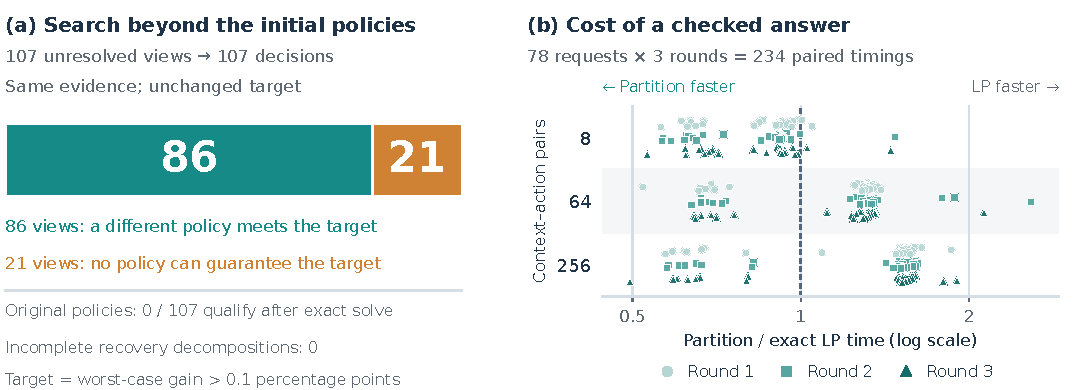
\includegraphics[width=\textwidth]{figures/verified_family_v7_main.pdf}
\caption{Checked cost and full-family search. (a) 26 requests per dimension $\times$ three dimensions $\times$ three rounds: all 234 pairs verify. Response time includes proof checking; offsets separate points. (b) Full-family search resolves all 107 remaining views (of 240): 86 admit a qualifying policy; 21 cannot support the guarantee. Exact rechecking of the original candidates recovers none. The decomposition separates tighter bounds from choosing a different policy. Rounds measure machine variation, not confidence intervals.}
\label{fig:complete-family}
\end{figure*}

\subsection{What complete family optimization adds}
\textbf{Broader policy search changes the fixed-view answer.}
The 240 primary finite Fusion views cover 48 worlds with five inference
samples each. Saved evidence settles 12 with above-threshold policies and
121 with zero capacity. Full search resolves the remaining 107 views:
86 admit new above-threshold policies; 21 have $0<\mathcal R\le\delta$,
excluding every such guarantee. Positivity alone therefore need not justify
further search. Overall, 98 views admit above-threshold policies and 142 do not.
Exact reoptimization of the original three policies recovers none of the 86:
their best value, including the reference, is zero in every case.
Recovered guarantees have median $0.991$\,pp, interquartile range
$[0.583,1.549]$\,pp and range $[0.105,3.632]$\,pp.
Only policy choice changes; information and views remain fixed.

Both methods agree on 2,160 unique synthetic requests (5,760 comparison positions).
Independent checking passes all 12,770/12,770 responses: 4,320 family responses,
7,762 fixed-policy optima, 220 Coat calls and 468 timing calls, without
timeout or incomplete call (Fig.~\ref{fig:complete-family}).

\textbf{Exact answers with dimension-dependent cost.}
All 234 timing pairs succeed. Across three rounds, construction/SoPlex
geometric-mean service ratios are $0.808$--$0.835$ at $d=8$,
$1.066$--$1.129$ at $d=64$, and $1.170$--$1.196$ at $d=256$.
The construction is slower in 5/78, 55/78 and 54/78 pairs, respectively.
These compare checked Python rational construction with compiled rational LP.
Pair costs, certificate sizes, memory observations and failure denominators
are archived. Table~\ref{tab:family-absolute} gives absolute costs.
At $d=256$, verification alone takes median 144.3/144.6\,ms (Part/LP);
certificates occupy about 149.5\,kB.
\begin{table}[t]
\centering\small
\caption{Medians over 78 calls per method/dimension. Response: after worker initialization through proof checking; Check: per-call receiver share; Whole: includes startup/cleanup. Part: partition construction; LP: SoPlex. kB: 1,000 bytes.}
\label{tab:family-absolute}
\begin{tabular}{@{}rr r r r r@{}}
\toprule
$d$ & Method & Response ms & Check \% & Whole ms & kB \\
\midrule
8 & Part & 4.66 & 24.4 & 122.2 & 3.47 \\
8 & LP & 4.99 & 22.1 & 135.2 & 3.47 \\
64 & Part & 53.58 & 23.2 & 172.2 & 20.93 \\
64 & LP & 40.85 & 31.6 & 170.0 & 20.91 \\
256 & Part & 648.13 & 22.8 & 770.3 & 149.51 \\
256 & LP & 419.97 & 34.6 & 554.0 & 149.44 \\
\bottomrule
\end{tabular}
\end{table}


\textbf{Source information is a separate comparison.}
At the larger R budget with conservative radius, projected R passes 223/240
thresholds versus Fusion's 218/240; R has greater capacity in 128 pairs,
Fusion in 100, with 12 ties. At the smaller R budget with oracle-boundary
radius, OBS and Fusion both pass 239 thresholds, but OBS has greater capacity
in 219 pairs and Fusion in 21. Full- and split-budget views are not nested.
All 24 comparison cells and exact decompositions remain available.
Generating means satisfy all 2,880 finite partition views, and every returned
policy assertion agrees with stored truth. These retrospective checks neither
establish uniform coverage nor validate source assumptions.


\subsection{The cost of answering repeated policy queries}
\begin{figure*}[t]
\centering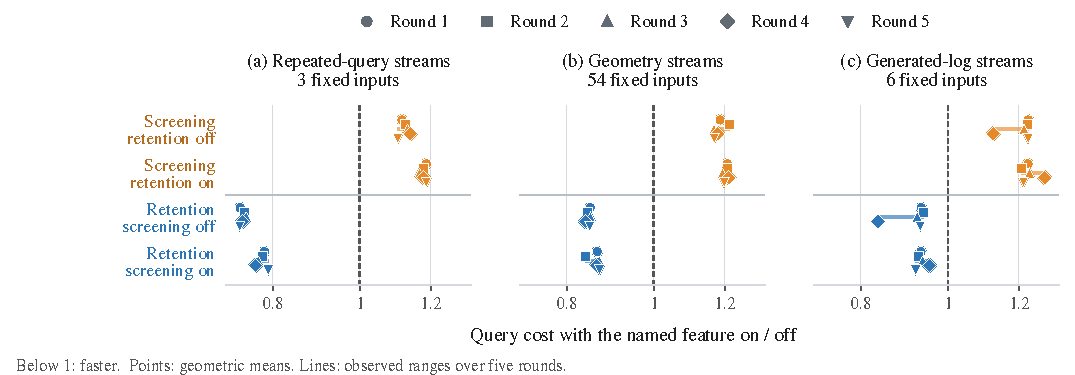
\includegraphics[width=\textwidth]{figures/optimized_v6_compact_factorial.pdf}
\caption{Retention lowers group-average cost; screening does not. Rows toggle the named feature while fixing the other off or on. Each point is one timing round's equal-input geometric mean of on/off cost ratios (R1--R5). Segments span the five rounds, not confidence intervals. The dashed line marks equal cost; below one is faster.}
\label{fig:optimized-factorial}
\end{figure*}
Retention saves the exact group terms that a new query would otherwise recompute; screening first tests whether an exact check can be deferred. All 270,000 responses pass independent exact replay; core plans match evidence,
decisions and native paths. Across the five primary rounds
(Fig.~\ref{fig:optimized-factorial}), retention ratios are
$0.735$--$0.748$ without screening and $0.766$--$0.791$ with it.
Screening ratios are $1.103$--$1.138$ without retention and
$1.165$--$1.186$ with it. Screening also costs more in every geometry and
source-derived group-round mean. Its earlier benefit without retention disappears under optimized arithmetic. Retention reduces cost with either screening setting in all five primary rounds.

The candidate-order control costs $0.833$--$0.882$ times $S_0P_1$ on primary streams,
but is slower in 1/15 primary, 66/270 geometry and 17/30 source-derived
input-round pairs. Retention also has adverse individual cases despite lower
group means. Thus retention lowers group-average cost without guaranteeing an individual speedup. Only this control changes candidate order.

\paragraph{Auxiliary execution controls}
Under fixed arithmetic, screening plus retention fails the registered joint-cost-ratio target $\leq0.8$ against each feature alone. Screening slows every broader-group round. A larger bank misses its speed target; changed decisions preclude isolated reuse attribution. Materialization helps ingestion, but preparation costs $1.580$/$1.619$ times hot execution under uniform/skewed assignment, respectively. Full controls remain in the artifact.


\subsection{Source information and query guarantees}\label{sec:information-results}
\begin{table}[t]
\centering
\caption{Projected Fusion: each row partitions 240 queries.}
\label{tab:fresh}\begingroup\small
\renewcommand{\arraystretch}{1.12}\setlength{\tabcolsep}{4pt}
\begin{tabular}{@{}lrrrr@{}}
\toprule
\rowcolor{QHeader}\qth{Policy} & \qth{Cert.} & \qth{Sampling} & \qth{Ambiguity} & \qth{True $\le\delta$}\\
\midrule
Metadata & 12 & 33 & 195 & 0\\
R heuristic & 4 & 43 & 190 & 3\\
Robust design & 2 & 0 & 0 & 238\\
\bottomrule
\end{tabular}\endgroup

\end{table}

Table~\ref{tab:fresh} follows three policies chosen before inference ($48$ worlds $\times5$ samples each); VI-A instead searches for a better policy on each fixed view. All 1,200 inference configurations across 60 worlds complete. For the metadata policy at $100d$ randomized events and $\Lambda=2$, fusion certifies 12/240 versus six for the standalone union (OBS six, R zero): six additions, no losses, certification-rate difference $0.025$ (2.5\,pp). The one-sided Hoeffding lower bound, $-0.3283$, does not meet the required $0.05$ increase; the descriptive $t$ interval is $[-0.0249,0.0749]$. These are changes in certification frequency, not policy gains. All six additions occur in two zero-drift $2\times4$ worlds.

Larger-budget projected fusion certifies 15 metadata, 16 heuristic and two robust-design queries; transfer and radius uncertainty remain.


\textbf{Why adding a source need not improve the bound.}\label{sec:budget-geometry}
For the same policy contrast $c$, fusion adds group constraints but splits the confidence budget. Let $\mathcal B_\alpha\subseteq\mathcal B_{\alpha/2}$ be full-budget OBS and fusion's observational box, with objective minima $B_\gamma=\min_{m\in\mathcal B_\gamma}c^\top m$. For nonempty $\C_F=\mathcal B_{\alpha/2}\cap\{a\le Tm\le b\}$, its optimum obeys
\begin{equation}
 V_F-B_{\alpha}=\underbrace{(V_F-B_{\alpha/2})}_{G\ge0}
                  -\underbrace{(B_{\alpha}-B_{\alpha/2})}_{P\ge0}.\label{eq:gain-cost}
\end{equation}
Fusion improves the full-budget observational bound exactly when its constraint gain $G$ exceeds its budget cost $P$.

\begin{proposition}[A checkable zero-gain condition]\label{prop:box-face}
Let $F_c=\arg\min_{m\in\mathcal B_{\alpha/2}}c^\top m$. Then $G=0$ if and only if $F_c$ contains a point satisfying all randomized group constraints. If $F_c$ is a singleton, checking its moment rows decides whether $G=0$ or $G>0$.
\end{proposition}
\noindent\textit{Proof.} A feasible box minimizer attains the box bound in $\C_F$. Conversely, compactness gives an optimizer in $\C_F$; equality places it in $F_c$. If the sets do not intersect, the gap is strict.\hfill$\square$

Choose box endpoints by the signs of $c$ and check the group rows. Feasibility proves zero constraint gain. If zero coefficients leave multiple minimizers, one failed point is inconclusive. We apply this test below.

\textbf{Sampling uncertainty versus ambiguity.}
Finite views include sampling uncertainty. Population views use exact generating statistics, but bias and transfer assumptions can still permit several target success-rate vectors. This remaining uncertainty is \emph{ambiguity}. For the metadata policy, all 240 true gains exceed $\delta$: 12 queries are certified, 195 are limited by ambiguity and 33 by sampling uncertainty (Table~\ref{tab:fresh}). Exact optima exclude optimization failure. Six additional finite certifications comprise four with sufficient standalone population information and two requiring fusion. At $100d$ R events, robust design retains the reference in 238/240 cases: true effect zero.

For the metadata policy, Fusion adds/loses 6/0, 9/0, 0/2 and 3/1 for $(\Lambda=2,100d)$, $(2,1000d)$, $(\Lambda^*,100d)$ and $(\Lambda^*,1000d)$, respectively; oracle $\Lambda^*$ comes from simulator truth. With $100d$ R events and oracle $\Lambda^*$, constraint gain averages 0.0114\,pp versus 0.0913\,pp budget cost. The zero-gain test holds for 193/240 queries, including both losses; the loss at $1{,}000d$ R events has positive gain below cost. All three losses persist at exact optima. Different samples and design policies prevent a causal sample-size interpretation.

\paragraph{Standalone-source controls}\label{sec:historical}
Observational consistency~\eqref{eq:consistency} lets OBS certify 99/100 external $2\times2$ queries; other policy/view settings differ. KuaiRec's imposed exposures and query-directed randomized means~\cite{gao2022kuairec} do not establish general complementarity: a 35-setting census finds no true-radius fusion-only case. 400 count/policy pairs remain in the artifact.




Additional checks cover three objects: 6,000 inference views have 14 coverage misses (outside the 2,880-view family subset) and no false certification; 18,900 final-mapping proofs all verify, leaving seven group-score certifications unresolved; 600 design views have one coverage miss.



\subsection{Real data: policy redesign and stopping}\label{sec:coat}
Here a policy chooses among 300 coat items for one user population ($K=1$), without personalization or a ranked list. The Coat dataset provides 24 self-selected and 16 randomly selected item ratings from each of 290 users~\cite{schnabel2016coat}. A success is a rating of at least four, not a purchase; zero entries denote unobserved ratings. Users, not the 11,600 ratings, are treated as independent. Within each source, potential ratings are assumed unaffected by presentation order or the other items in a user's panel.

Group constraints use \emph{item} attributes: gender category, jacket type and color. Their separate partitions total 31 rows and overlap when combined. Twelve assumption settings cross $\Lambda\in\{1,1.5,2,3\}$ with $\rho\in\{0,.02,.05\}$; the primary setting is $(2,0)$. Fifteen candidate policies upweight or downweight front-page, men's, fleece, waterproof or black items: $\pi_i\propto t^{h_i}$ for binary attribute $h_i$ and $t\in\{.5,1.5,2\}$. The reference selects uniformly ($1/300$); the primary candidate doubles front-page item weights, then normalizes. Only the three front-page policies have contrasts outside the span of group rows.

To use all ratings, we assume each user's 16 R items form a simple random subset independent of potential ratings. The release describes random/uniform selection; collection code is unavailable. A control retains one rating per source/user without looking at its value, giving $q_a=(16/300)/16=1/300$. Its 580 events leave 116 empty O and 124 empty R cells; none of 900 queries or 15 full-cell controls is certified. Discarding the panels loses substantial information.

Inference accounts for repeated ratings. O intervals count included users per item; joint bounds use $N=290$. Uniform thinning divides inclusion probabilities by 24, preserving their ratio and $\Lambda$, but weakens consistency bounds. For R group scores, each user averages their ratings within a group. Under the subset assumption this is an unbiased group-mean estimate; the 72--290 active-user scores lie in $[0,1]$ and enter~\eqref{eq:eb}. Their sample variance uses $n_j-1$ and requires user-level records. Projected intervals instead use per-item CP and propagate through~\eqref{eq:represented}.


\begin{table}[t]
\centering
\caption{Coat: one policy versus the full policy family.}
\label{tab:coat-blocks}\begingroup\small
\renewcommand{\arraystretch}{1.14}\setlength{\tabcolsep}{2pt}
\begin{tabular*}{\columnwidth}{@{\extracolsep{\fill}}lrrrr@{}}
\toprule
& \qth{\shortstack{Fixed policy\\Primary setting}} & \multicolumn{3}{c}{\qth{\shortstack{Full policy family\\Assumption settings}}}\\
\cmidrule(lr){2-2}\cmidrule(lr){3-5}
\qth{Construction} & \qth{LCB (pp)} & \qth{Zero} & \qth{Small} & \qth{Qualifies}\\
\midrule
OBS & $-3.729$ & 9/12 & 0/12 & 3/12\\
R group & $-1.502$ & 12/12 & 0/12 & 0/12\\
R projected & $-3.402$ & 12/12 & 0/12 & 0/12\\
\addlinespace[2pt]
Fusion group & $-1.193$ & 7/12 & 1/12 & 4/12\\
Fusion projected & $-3.132$ & 9/12 & 3/12 & 0/12\\
\midrule
R full-cell control & $-3.077$ & 1/1 & 0/1 & 0/1\\
\bottomrule
\end{tabular*}\endgroup\par
\smallskip
\parbox{\columnwidth}{\footnotesize\raggedright
LCB: one fixed policy at primary $(\Lambda,\rho)=(2,0)$, in pp. Family columns: $\mathcal R=0$, $0<\mathcal R\le\delta$, or $\mathcal R>\delta$ across twelve settings on the same 290 users. All five primary capacities are zero. Full-cell transport is a stronger, one-setting control. Here $\alpha=.05$, $\delta=.001$ (0.1\,pp).}

\end{table}

% Generated from independently audited fixed-data V5 repair.
All 915 fixed-policy lower-bound queries are unresolved, with no refused view.
At the primary declaration, group Fusion improves the bound over full-budget
R group by 0.309\,pp, but neither passes $\delta=.001$ (Table~\ref{tab:coat-blocks}).
Independent audit reconstructs user statistics, 61 views, 915 proofs and
15 direct controls; it does not establish the source assumptions.


\textbf{Deciding beyond the tested policies.}
With the normalized ideal reference $1/300$, complete family optimization
resolves all 60 original grid positions: 49 have $\mathcal R=0$, four have
$0<\mathcal R\le.001$, and seven have $\mathcal R>.001$.
The seven positive declarations represent five unique mathematical requests:
OBS at $\Lambda=1$ repeats across three tolerances; group Fusion passes at
$\Lambda=1$ for all three tolerances and at $\Lambda=1.5,\rho=0$.
These supply checked policies although the original fifteen-candidate
evaluation certified none, conditional on the stated assumptions; there is
no joint guarantee across declarations.

\textbf{A concrete policy decision.}
At $\Lambda=1.5,\rho=0$, the jacket-type certificate reallocates all 28 vests'
uniform mass to item 0, a men's bomber: its probability rises from $1/300$ to
$29/300$, the vests receive zero, and 271 items stay at $1/300$.
All 15 original and 50 extended catalogue policies retain full support,
so none makes this choice. The contrast is
$(28/300)(m_0-\overline m_{\rm vest})$, with $\overline m_{\rm vest}$ the
uniform mean of the 28 vests. Its checked lower bound is
$(28/300)(\ell_0-b_{\rm vest}/\kappa_{\rm vest})$: the stored row mass
$\kappa$ converts the group constraint to its uniform mean.
Only these two terms are nonzero, contributing $2.472638$\,pp and
$-2.226283$\,pp, respectively.
Their sum guarantees $0.246355$\,pp in expected high-rating probability
over uniform, exceeding $0.1$\,pp and matching the full overlapping view's
capacity. Matched full-budget OBS and both R views have zero capacity.
This retrospective answer assumes confounding no greater than $\Lambda=1.5$
and no group-mean drift. It neither selects those assumptions from data nor
measures purchase uplift; it does not imply every vest is worse.

All five primary $\Lambda=2,\rho=0$ views still have zero capacity. In group
Fusion, every item mean can equal $0.2186$ (rounded), tying every policy with
the reference. A checked constant point already supplies this stopping answer;
it is not an exclusive benefit of full optimization. The stronger full-cell
control also has zero capacity.

The natural gender, jacket-type and color partitions supply 144 memberships:
10 exceed the threshold, 10 have positive capacity at most the threshold, and
124 have zero capacity. The construction and exact LP agree on all 95 unique
supported requests across the full evaluation; the LP additionally resolves
30 overlapping requests. Every partition subview has capacity at most its
parent's, as required by relaxation. These are dependent views of one dataset,
not 144 independent experiments or new evidence for sampling assumptions.


% Estimator description checked against the saved user-level direct control.
Under full-cell transport, each user's score is $Z_u=(300/16)\sum_{a\in S_u}c_aY_{ua}$, with random panel $S_u$, binary high-rating outcomes $Y_{ua}$ and policy contrast $c=\pi-\pi_0$. The factor $300/16$ corrects each item's inclusion probability $16/300$. A one-sided Hoeffding bound across 290 users uses score range $[\min(0,300\min c),\max(0,300\max c)]$. The primary estimated gain over uniform is $0.371$\,pp, with lower bound $-6.452$\,pp; none of 15 fixed queries passes. These bounds cover each prespecified query separately.


\label{sec:catalogue-workflow}
\paragraph{Catalogue queries with ordinary caching}
For each primary Coat view, combine two of the five indicators:
$\pi_i\propto t_1^{h_{1i}}t_2^{h_{2i}}$, with
$(t_1,t_2)\in\{.5,1,2\}^2\setminus\{(1,1)\}$.
Ten pairs give 80 policy positions at margins $0,.001,.01$ (0, 0.1, 1\,pp):
240 requests, 50 distinct objectives and 150 objective--margin pairs.
Prepared execution retains exact dual terms; optimized-exact adds sparse
arithmetic and cached number conversions. Both share full objective caching
and a persistent receiver. Native hot-start retains a solver basis without
cross-objective certificate candidates. Quality checks precede three timing rounds.

Prepared and optimized-exact agree on all 1,200 requests, but cost ratios
$0.960$, $0.941$, $0.953$ miss the ten-percent target. Optimized-exact is slower
in 3/15 view-rounds and retains more estimated exact-state payload in every
view (not isolated RSS). Native hot-start changes 98 false answers to unknown
and four unknown answers to false; it never reverses a Boolean answer.
Thus overall service differs; on R projected, decisions agree and native is
faster in all rounds. None certifies improvement, and neither fusion-only
information target is supported. The five views have zero capacity, so a
constant-action witness can already justify stopping.

\paragraph{The cost of family preprocessing}
This experiment tests whether family evidence accelerates the unchanged
catalogue. A useful policy outside it can coexist with false answers inside it.
We repeat the 240 queries on two 16-row jacket-type Fusion
views, $(\Lambda,\rho)=(1.5,0)$ and $(2,0)$, selected retrospectively with known
capacities. Hot-start (Hot), optimized threshold execution (Opt), and Opt with
partition (Part) or exact-LP (LP) preprocessing share objective caching, checked
points and a rational receiver. Family certificates add only feasible points;
a shared constant-action shortcut skips unnecessary family solves.
Unresolved represented queries permit one producer attempt per objective--margin
pair and one complete exact fallback per objective; ideal answers reuse this
evidence without extra solves.

\begin{table}[t]
\centering
\caption{Original Coat queries. Time: median seconds over three rounds, including
startup, family work, external verification and cleanup. Ratio/Opt: paired
cost range (above one is slower). N/E/F: native/fixed-exact/family calls,
identical per stream across quality and timing. Both views use $\rho=0$.}
\label{tab:coat-workflow}
\begingroup\small
\renewcommand{\arraystretch}{1.10}\setlength{\tabcolsep}{4pt}
\begin{tabular}{@{}llrrr@{}}
\toprule
\rowcolor{QHeader}\qth{View} & \qth{Plan} & \qth{Time (s)} & \qth{Ratio/Opt} & \qth{N/E/F} \\
\midrule
$\Lambda=1.5$ & Hot & 6.800 & 0.974--1.009 & 2/2/0 \\
$\Lambda=1.5$ & Opt & 6.934 & 1.000 & 2/2/0 \\
$\Lambda=1.5$ & Opt+Part & 7.312 & 1.051--1.077 & 2/2/1 \\
$\Lambda=1.5$ & Opt+LP & 7.276 & 1.042--1.079 & 2/2/1 \\
\midrule
$\Lambda=2$ & Hot & 6.329 & 0.985--0.998 & 1/1/0 \\
$\Lambda=2$ & Opt & 6.390 & 1.000 & 1/1/0 \\
$\Lambda=2$ & Opt+Part & 6.431 & 0.999--1.024 & 1/1/0 \\
$\Lambda=2$ & Opt+LP & 6.359 & 0.990--1.002 & 1/1/0 \\
\bottomrule
\end{tabular}\endgroup

\end{table}

All 32 streams complete, each with 240 false answers under both semantics.
On the nonzero-capacity view, Part adds 5.1--7.7\% to Opt's full cost without
reducing its two native and two exact calls (Table~\ref{tab:coat-workflow});
LP likewise saves no calls. The zero-capacity control skips family computation.
Three rotations describe machine variation; execution positions are not fully
balanced. Different optimal points compare complete preprocessing choices.
Family answers enable redesign beyond the catalogue but do not amortize
preprocessing here.


\section{Related Work and Scope}\label{sec:related}
\textbf{Database queries.} Causal systems adjust aggregates~\cite{salimi2018hypdb}, implement matching~\cite{salimi2017zaliql}, define units~\cite{salimi2020carl} and explain patterns~\cite{youngmann2024causumx}. Uncertainty-annotated databases propagate bounds~\cite{Feng2019UADB}; semantic views certify predicates using fresh draws~\cite{Hassanzadeh2026SemanticViews}. Q-BRIDGE materializes source-dependent constraints once and evaluates changing policy objectives over their shared feasible set. Its additional query is whether any policy can meet a guarantee; matching certificates verify that answer and reusable terms reduce repeated arithmetic.

Our view combines binary density-ratio and conditional-moment relaxations~\cite{dorn2025dvds,ishikawa2026convex}. Other fusion methods exploit overlap~\cite{jiang2024overlap}, impose experimental moments~\cite{du2026feasible}, or estimate sensitivity frontiers~\cite{lanners2025fusion}. Propensity-odds policy learning~\cite{Kallus2018ConfoundingRobust,Hess2026SharpPolicy} makes different restrictions from our outcome-conditional weights.
\par\textbf{Classical allocation.} Continuous maximin sharing~\cite[Sec.~2.2]{Yamada1998Sharing} allocates a common resource across groups. Our groups instead impose disjoint, two-sided constraints on uncertain means; we minimize the best action's advantage over a reference and recover an original-constraint certificate.


\textbf{Proofs and scope.} Filtering~\cite{Bartels2023Filters}, assignment caching~\cite{Cadar2008KLEE}, bounds and reuse are established; VIPR checks exact optimization proofs~\cite{Cheung2017VIPR}. IntegriDB authenticates results~\cite{Zhang2015IntegriDB}; our digests bind certificates to a view. Our guarantees cover binary outcomes and known target weights under the stated source assumptions and intervals.

\textbf{Data ethics.} We reanalyze public benchmarks under their release terms, without recruiting or contacting participants. No institutional ethics review was undertaken or additional consent sought.

\section{Conclusion}
Q-BRIDGE turns integrated, uncertain evidence into a reusable object for policy queries. One coverage event supports changing objectives; matching certificates establish whole-family answers, and exact-term reuse reduces repeated-query cost. Coat distinguishes stopping on an exhausted view from redesign under an explicitly stronger declaration.

\clearpage
\section*{Acknowledgments and AI Usage Declaration}
The authors conceived the research, designed the overall study, and led the manuscript writing. OpenAI Codex assisted with drafting, polishing and mathematical exposition (Sections I--VIII), code and experiments (Sections III--VI), figures, and source retrieval. The authors take full responsibility for the manuscript, including any text generated or polished by the LLM, and for ensuring its accuracy, originality, proper attribution, and compliance with publication ethics, including the prevention of plagiarism and scientific misconduct.

\bibliographystyle{IEEEtran}
\bibliography{revision7_references}
\end{document}
